\documentclass[a4paper,12pt]{article}
\usepackage[utf8]{inputenc}
\usepackage[brazilian]{babel}
\usepackage{color}
\usepackage{graphicx}
\usepackage{subfig}
\usepackage[hmargin=2cm,vmargin=3.5cm,bmargin=2cm]{geometry}
\usepackage{cite}
\usepackage{float}
\usepackage{enumerate}
\usepackage{amsmath}
\usepackage{verbatim}

\begin{document}

\title{}

\author{Aluno: Rafael M. Miller NUSP.: 7581818}

\maketitle

\section{Introdução}

\begin{equation}
\varepsilon_n = \frac{E_{tubo} sen(n \Delta \phi) \zeta(n)}{n E_{fundo} \pi R^{n+2} + n  E_{tubo} \Delta \phi \zeta(n)}
\label{eq:analitical_epsilon_n}
\end{equation}



\begin{figure}[H]
\centering

\subfloat[]{
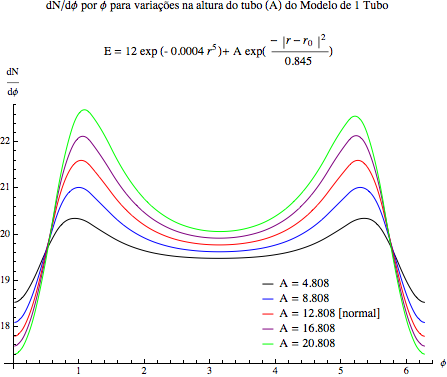
\includegraphics[scale=0.65]{variaA.png}
}
\subfloat[]{
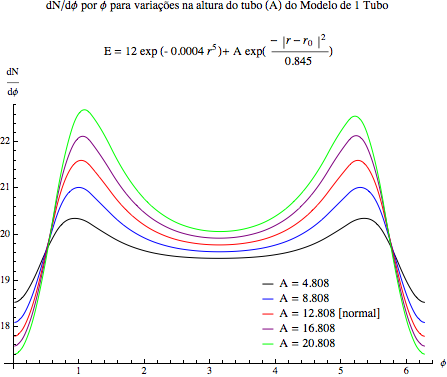
\includegraphics[scale=0.58]{variaA.png}
}
\caption{Gráficos da aproximação realizada na condição inicial conhecida por Modelo de 1 Tubo dada pela equação (\ref{eq:1tubo}) e apresentada no gráfico da Figura \ref{fig:CINeXusE1Tubo}.b. Para este exemplo foi utilizado $r_0 = 4,4 fm$. (a): Perfil de densidade de energia (E) pelo raio (r) em $\phi = 0$, em vermelho está apresentado o Modelo de 1 Tubo calculado por (\ref{eq:1tubo}) e, em azul, a aproximação por constantes. (b): Corte transversal da condição inicial aproximada por constantes.}
\label{fig:AproxModelo1Tubo}
\end{figure}

\section{Desenvolvimento e Análises}



\begin{thebibliography}{99}

\bibitem{rhic}
Relativistic Heavy Ion Collider website: \verb#http://www.bnl.gov/rhic/#

\bibitem{lhc}
Large Hadron Collider website: \verb#http://home.web.cern.ch/topics/large-hadron-collider#

\bibitem{weinberg}
Steven Weinberg. Três Primeiros Minutos, Os. Gradiva, 1987

\bibitem{spherio}
Y. Hama, T. Kodama, O. Socolowski, Jr., Braz. J. Phys. \textbf{35}, 24 (2005).

\bibitem{Jaki}
J. Noronha-Hostler, G. S. Denicol, J. Noronha, R. P. G. Andrade, F. Grassi, Phys. Rev. C \textbf{88}, 044916 (2013) [arXiv:1305.1981 [nucl-th]].

%\bibitem{gubser}
%S. S. Gubser, Phys. Rev. D \textbf{82}, 085027 (2010) [arXiv:1006.0006 [hep-th]].

%\bibitem{bjorken}
%J. D. Bjorken, Phys. Rev. D \textbf{27}, 140 (1983).

%\bibitem{noronha}
%H. Marrochio, J. Noronha, G. S. Denicol, M. Luzum, S. Jeon, C. Gale [arXiv:1307.6130 [nucl-th]]

\bibitem{nexus}
T. Pierog, M. Bleicher, K. Mikhailov, K. Werner, I. Karpenko. Phys. Rev. C \textbf{82}, 044904(2010). [arXiv:1004.0805 [nucl-th]].

\bibitem{glauber}
H.-J. Drescher, Y. Nara, Phys. Rev. \textbf{C 75}, 034905 (2007); 76, 041903 (2007)

\bibitem{1tubo1}
Y. Hama, R. P. G. Andrade, F. Grassi, W. L. Qian, Nonlin. Phenom. Complex. Syst. \textbf{12}, 466(2009). [arXiv:0911.0811 [hep-ph]].

\bibitem{1tubo2}
R. P. G. Andrade, F. Grassi, Y. Hama, W. L. Qian, Physics Letters. B, \textbf{712} [arXiv:1008.4612 [nucl-th]].

\bibitem{fernando}
F. G. Gardim, F. Grassi, M. Luzum , J-Y. Ollitrault, Phys. Rev. C \textbf{85}, 024908 (2012) [arXiv:1111.6538 [nucl-th]]

%\bibitem{cooperfrye}
%F. Cooper and G. Frye, Phys. Rev. D \textbf{10}, 186 (1974).

%\bibitem{Romatschke}
%Romatschke, P., Int.J.Mod.Phys.\textbf{19} 1-53 (2010), arXiv:0902.3663v3 [hep-ph]

%\bibitem{nobel}
%``The Nobel Prize in Physics 2013". Nobelprize.org. Nobel Media AB 2014. Web. 17 Jul 2014. \verb#http://www.nobelprize.org/nobel_prizes/physics/laureates/2013/#

\end{thebibliography}

\end{document}
